\section{Rete neurale}
\label{Rete neurale}

La libreria utilizzata per sviluppare la Rete neurale \`e stata \textit{ConvNetJS}. L'aspetto positivo di tale scelta \`e stata la semplicit\`a nell'utilizzo del linguaggio javascript; l'aspetto negativo ha riguardato la totale mancanza di mantenibilit\`a della libreria stessa che comporta la scarsit\`a di esempi applicativi, oltre alla documentazione ufficiale, che costringono lo sviluppatore ad una ricerca approfondita personale in un ambiente ove lo nozioni si presentano scarse e a continue prove per verificare la validit\`a del codice prodotto.
\begin{figure}[H]
\centering
	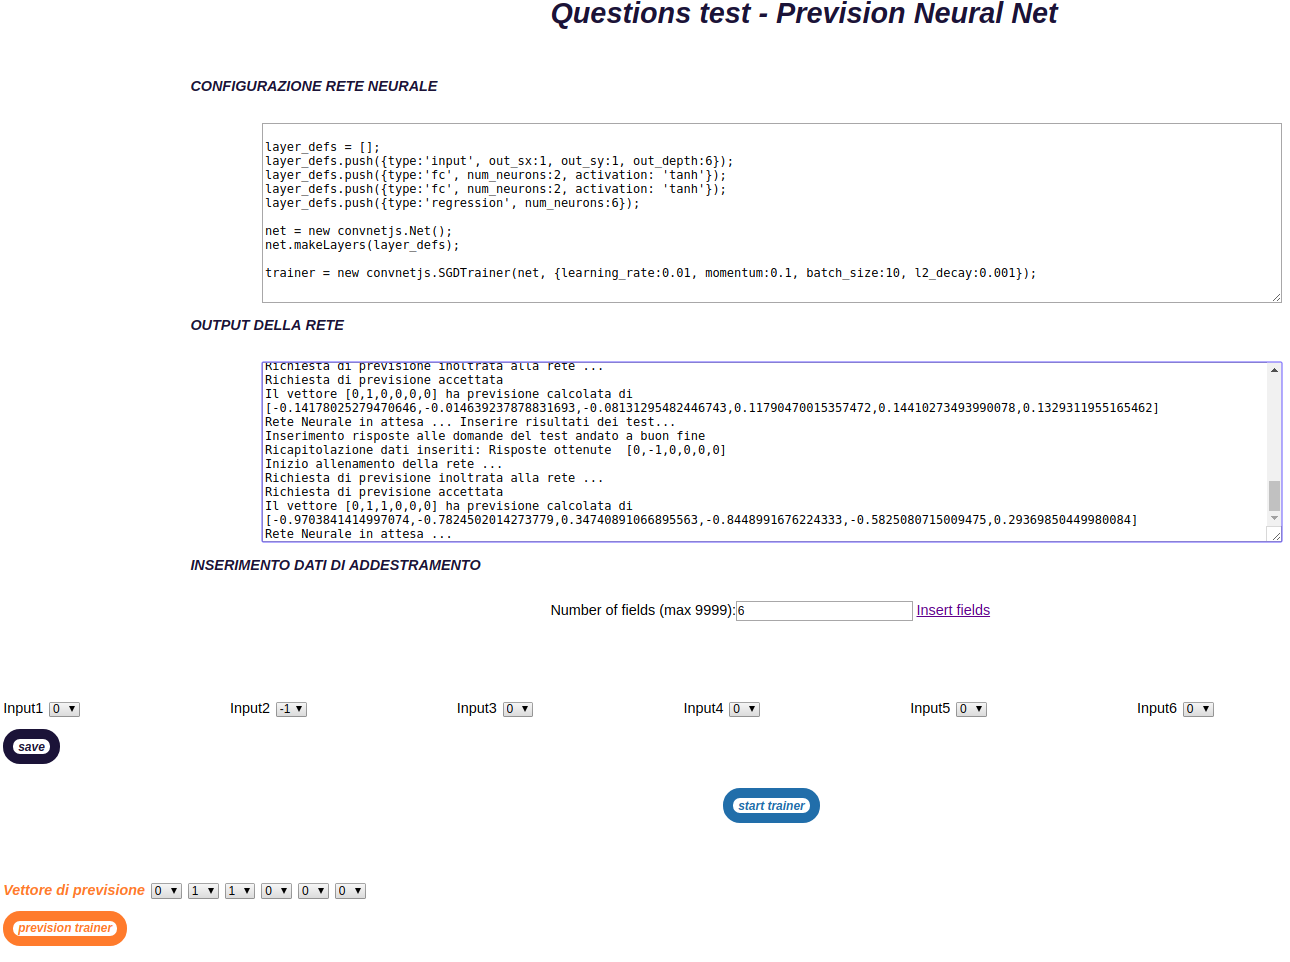
\includegraphics[width=1\linewidth]{./image/GUI-rete-neurale.png}
	\caption{Interfaccia utente della Rete neurale di prova.}
\end{figure}
\noindent
Durante il periodo 24/05 - 31/05 mi sono occupata dello sviluppo di una Rete neurale in grado di ricevere in input un training set di dimensione 6 e di restituire una previsione sui dati di apprendimento ricevuti.
\noindent
Il problema che la rete mira ad analizzare \`e quello discusso nel precedente capitolo \textit{Analisi dei dati di probabilit\`a}
\\\\
Per aggevolare l'apprendimento della rete, ed ottenere delle previsioni stabili mi sono occupata di implementare due metodi di generazione randomica di dati in modo da far apprendere massiciamente la stessa.
Il dato prodotto consiste in un vettore di 6 elementi, composto da  -1, 0 e 1 con il seguente criterio:
\begin{itemize}
\item \textbf{-1}: la domanda x \`e stata posta al candidato che ha risposto in maniera errata;
\item \textbf{0}: la domanda x non \`e stata posta al candidato;
\item \textbf{1}: la domanda x \`e stata posta al candidato che ha saputo rispondere correttamente.
\end{itemize}
\noindent
Il primo metodo che ho sviluppato si occupa di generare un vettore di dati di apprendimento basandosi esclusivamente su come le domande sono interconnesse tra di loro (grazie all'uso di un grafo della conoscenza costruito ad hoc); il secondo metodo ripropone quanto perseguito dal primo metodo con il valore aggiunto di generazione di un profilo randomico di un candidato, che tiene conto della  probabilit\`a di risposta ad una domande seguendo la formula P(A)= $\frac{1}{3}+\frac{1}{6}P(S_1)+\frac{2}{3}P(S_2)$.

\subsection{Test effettuati}
\label{Test effettuati}

Alcune decisioni che ho preso durante la configurazione della rete riguardano i seguenti settori:
\begin{enumerate}
\item Una rete neurale non deve, per fornire dei dati attendibili, possedere un numero di neuroni troppo elevato rispetto al trainset effettuato; altrimenti la previsione  ritornerebbe l'identit\`a del vettore di input della stessa, come conseguenza diretta della capacit\`a troppo elevata di immagazzinare dati.
\item I layers, ho deciso, di allenarli mediante tecnica di regressione, che permette l'inserimento in input di una funzione obiettivo e l'ottenimento di un risultato, in output, anche in virgola mobile e composto di tanti elementi quanti sono i neuroni di regressione dichiarati. Per la mia rete di prova \`e necessario dichiarare  6 neuroni in regressione perch\`e l'output, appunto, che ci si aspetta dal sistema \`e di 6 elementi.
\item Per costruire un dataset di dati consistente che permettesse alla rete di imparare qualcosa ho costruito un grafo della conoscenza con lo scopo di mettere in relazione degli argomenti che coinvolgono uno o pi\`u domande.
\begin{figure}[H]
\centering
	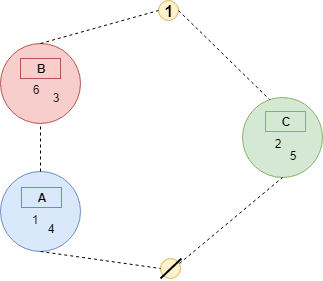
\includegraphics[width=0.60\linewidth]{./image/grafo_trainset.png}
	\caption{Grafo rappresentante le relazioni esistenti tra il set di domande di prova.}
\end{figure}
\noindent
Per svolgere l'apprendimento ogni vettore, facente parte del dataset, viene dato in pasto alla rete che a sua volta provvede alla sua assimilazione come conoscenza mediante la tecnica dell'autoencoder, ovvero la rete impara il vettore riducendone lo spazio occupato.
\item Per creare il dataset ho ritenuto sufficiente generare \textit{2000} vettori di risposta in modo da compiere in maniera esaustivo l'apprendimento della rete.
\end{enumerate}
\noindent
Il vettore passato in input per svolgere le previsioni \`e \textit{[0,1,0,0,0,0]}\\
\noindent. 
Di seguito riporto quanto \`e stato rilevato in fase di test.

\subsubsection{Configurazione della rete: 4 neuroni per ciascuno dei 2 layers}
\label{Configurazione della rete: 4 neuroni per ciascuno dei 2 layers}

Configurazione della rete utilizzata:\\
\begin{verbatim}layer_defs = [];
layer_defs.push({type:'input', out_sx:1, out_sy:1, out_depth:6});
layer_defs.push({type:'fc', num_neurons:4, activation: 'tanh'});
layer_defs.push({type:'fc', num_neurons:4, activation: 'tanh'});
layer_defs.push({type:'regression', num_neurons:6});

net = new convnetjs.Net();
net.makeLayers(layer_defs);

trainer = new convnetjs.SGDTrainer(net, {learning_rate:0.01,
 momentum:0.1, batch_size:10, l2_decay:0.001});
\end{verbatim}
\noindent
I layers utilizzati sono 2 e compositi da 4 neuroni.

\paragraph{Training set standard a 4 neuroni per ciascuno dei 2 layers}\mbox{}
\label{Training set standard a 4 neuroni per ciascuno dei 2 layers}
\\
\noindent
\begin{itemize}
\item \begin{verbatim}[0.06185960218322828,-0.27133263709888233,0.11724865743521667,
-0.03165246440684366,0.0930428691265781,-0.4358467270595998] \end{verbatim}
Appaiono in relazione le domande 1, 3, 5 e 2, 4, 6.\\
Gli scostamenti tra le coppie 2 e 5, 1 e 4, 3 e 6 non sono consistenti con quelle che sono le relazioni di dipendenza,\`e una differenza che parte da qualche millesimo fino 0.5 circa; che mi sembra troppo per venire associata solamente alla presenza di valori -1 all'interno del vettore di training.
Le domande 3 e 6 si dovrebbero presentare con una positivit\`a inferiore rispetto a 1 e 4; nel test in analisi questo viene rispettato solo dalle coppie 1, 6 e 4, 6  per una differenza trascurabile attorno allo 0.1.

\item \begin{verbatim}[0.0591737964385515,0.04700554500974672,0.1770953961599532,
-0.032873052126447984,-0.21556028214336714,0.05438007273096417]\end{verbatim}\\
Appaiono in relazione le domande 1, 2, 3, 6 e 4, 5.\\
Gli scostamenti tra la coppia 3, 6 sono consistenti con quelle che sono le relazioni di dipendenza fra le domande; invece per quanto concerne le coppie 1, 4 e 2, 5 hanno una differenza che oscilla da qualche millesimo fino a 0.2, che mi sembra adeguata dalla presenza di -1  all'interno dei vettori di training.
Le domande 3 e 6 si dovrebbero presentare con una positivit\`a inferiore rispetto a 1 e 4; nel test in analisi questo vale per le coppie 1, 6; in tutti gli altri casi vi \`e una differenza trascurabile di qualche millesimo.

\item \begin{verbatim}[0.24761793901633827,-0.006279637560350819,-0.05180076990401846,
0.1813232184712338,-0.057742845674898,0.07468235957894961]
\end{verbatim}\\
Appaiono in relazione le domande 1, 4, 6 e 2, 3, 5.\\
Gli scostamenti tra le  coppie 1, 4 e 2, 5 sono consistenti con quelle che sono le relazioni di dipendenza fra le domande; invece per quanto concerne le coppia 3, 6 vi \`e una differenza attorno allo 0.012 circa; che mi sembra adeguata alla presenza di valori -1 all'interno del vettore di training.
Le domande 3 e 6 si dovrebbero presentare con una positivit\`a inferiore rispetto a 1 e 4; nel test in analisi solo la regola viene rispettata pienamente.

\item \begin{verbatim}[-0.41386243742641304,0.2293601640299243,-0.15172273330068514,
-0.08993270051292439,-0.16696727087969201,-0.030153227547984836]\end{verbatim}
Appaiono in relazione 1, 3, 4, 5, 6 e 2 (a parte).\\
Gli scostamenti tra le coppie 2 e 5 non sono consistenti con quelle che sono le relazioni di dipendenza fra le domande per una differenza attorno allo 0.2 circa.
Le domande 3 e 6 si dovrebbero presentare con una positivit\`a inferiore rispetto a 1 e 4; nel test in analisi solo dalle coppie 4, 3 e 4, 6; in tutti gli altri casi la differenza oscilla da uno 0.25 ad uno 0.4 circa che mi sembra troppo da associare esclusivamente alla presenza di valori -1 nel set di training.
\end{itemize}


\paragraph{Training set con generazione del profilo di un candidato e calcolo delle probabilit\`a di risposta a 4 neuroni per ciascuno dei 2 layers}\mbox{}
\label{Training set con generazione del profilo di un candidato e calcolo delle probabilita di risposta a 4 neuroni per ciascuno dei 2 layers}
\\
\noindent
\begin{itemize}
\item  \begin{verbatim}[0.12233318607288908,0.11271870424991579,0.03946474842257475,
0.010689268243140052,-0.2212488419725651,0.08871808059256903]
\end{verbatim}
Appaiono in relazione le domande 1, 2, 3, 4, 6 e 5 (a parte).\\
La coppia 2, 5 non \`e in relazione stretta con una differenza dello 0.3 circa. La domanda 4 presenta con una positivit\`a inferiore rispetto alla domanda sia 3 che 6 non mostrandosi cos\`i conforme alla regola per una differenza trascurabile attorno a qualche millesimo, invece la domanda 1 risulta conforme. L'anomalia pu\`o venire ricondotta all'uso di un set con dati "spuri", calcolati mediante la probabilit\`a che un candidato ha di rispondere correttamente o meno ad una i-esima domanda (tale formula ha fatto venire meno la validit\`a parziale delle relazioni che intercorrono tra le domande) che alla presenza dei valori -1 del vettore di training. Il secondo fattore per\`o ha sicuramente un influenza inferiore rispetto al primo sui risultati ottenuti.

\item \begin{verbatim}[0.10964014479802053,0.1858249376842786,-0.5006601985527853,
-0.0334676581944329,-0.09971574849174258,-0.3801105216529717]

\end{verbatim}
Appaiono in relazione le domande 1, 2  e 3, 4, 5, 6.\\
Le coppia 2, 5 e  1, 4 non \`e pi\`u in relazione stretta ma con una differenza 0.2 - 0.5; questo non vale per la coppia 3, 6 che rimane conforme alla regola. Sia la domanda 1 che 4 si presentano in rapporto con la domanda 3 e 6 con positivit\`a superiore conforme alla regola. 
Le anomalie riscontrate possono venire ricondotte all'uso di un set con dati "spuri", calcolati mediante la probabilit\`a che un candidato ha di rispondere correttamente o meno ad una i-esima domanda (tale formula ha fatto venire meno la validit\`a parziale delle relazioni che intercorrono tra le domande) che alla presenza dei valori -1 del vettore di training. Il secondo fattore per\`o ha sicuramente un influenza inferiore rispetto al primo sui risultati ottenuti.

\item  \begin{verbatim}[0.6928150525498127,-0.12346483511365285,0.3519927766897261,
-0.29213616574371004,-0.2664118985214089,-0.4278610241686793]
\end{verbatim}
Appaiono in relazione le domande 1, 3 e 2, 4, 5, 6.\\
La coppia 1, 4 non \`e pi\`u in relazione stretta ma con una differenza importante che oscilla attorno allo 0.8 circa. La domanda 1 presenta una positivit\`a superiore rispetto alla domanda alla 3 e 6, mostrandosi  conforme alla regola; invece la domanda 4 ha una differenza  attorno allo 0.6 - 0.8. L'anomalia pu\`o venire ricondotta all'uso di un set con dati "spuri"  usati per effettuare il training degli stessi.

\item  \begin{verbatim}[-0.36082231867252107,-0.04413191737526341,0.5586488173865226,
0.7496419035838204,-0.3774536487859032,0.20900746632808334]
\end{verbatim}
Appaiono in relazione le domande 1, 2, 5 e 3, 4, 6.\\
Le domanda 2, 5 e 3, 6  sono in relazione stretta, questo non vale per la coppia 1, 4 che ha una differenza che supera l'unit\`a. La domanda 4 presenta una positivit\`a superiore rispetto alla domanda sia 3 che 6  dimostrandosi conforme alla regola; negli altri casi la differenza si attesta attorno con una differenza attorno 0.6 - 0.8. L'anomalia pu\`o venire ricondotta all'uso di un set con dati "spuri" usati per il effettuare il training degli stessi.
\end{itemize}

\paragraph{Osservazioni}\mbox{}
\label{Osservazioni su rete a 4 neuroni per ciascuno dei 2 layers}
\\\\
\noindent
La configurazione testata si compone di 4 neuroni a layer su una base di 2000 test correndo il rischio di avere una rete che apprende troppo e come effetto negativo "veda" addirittura cose che non esistono.\\
Per fare un 'ulteriore verifica del sistema da me sviluppato ne ho mutato la configurazione riducendo il numero di neuroni presenti in ciascun layers e/o il numero di layers presenti.\\
Le nuove configurazione su cui ho effettuato i test sono esposte nei paragrafi seguenti.

\subsubsection{Configurazione della rete a 2 neuroni per ciascuno dei 2 layers}
\label{Configurazione della rete a 2 neuroni per ciascuno dei 2 layers}
Configurazione della rete utilizzata:\\
\begin{verbatim}layer_defs = [];
layer_defs.push({type:'input', out_sx:1, out_sy:1, out_depth:6});
layer_defs.push({type:'fc', num_neurons:2, activation: 'tanh'});
layer_defs.push({type:'fc', num_neurons:2, activation: 'tanh'});
layer_defs.push({type:'regression', num_neurons:6});

net = new convnetjs.Net();
net.makeLayers(layer_defs);

trainer = new convnetjs.SGDTrainer(net, {learning_rate:0.01,
 momentum:0.1, batch_size:10, l2_decay:0.001});
\end{verbatim}
\noindent
I layers utilizzati sono 2 compositi da 2 neuroni.

\paragraph{Training set standard su rete a 2 neuroni per ciascuno dei 2 layers}\mbox{}
\label{Training set standard su rete a 2 neuroni per ciascuno dei 2 layers}
\\
\noindent
\begin{itemize}
\item \begin{verbatim}[0.21244167155728633,0.3163244589382085,0.5553080475586194,
0.9592565134409513,-0.4523485201932427,0.05451735176218134]\end{verbatim}
Appaiono in relazione le domande 1, 2, 3, 4, 6 e 5 (a parte).\\
Gli scostamenti tra le coppie 1, 4 e 3, 6 sono consistenti con quelle che sono le relazioni di dipendenza fra le domande; invece per la coppia 2, 5 i segni sono opposti con una differenza dello 0.8, che posso far ricondurre alla presenza dei valori -1 nel vettore di training.
Le domande 3 e 6 si dovrebbero presentare con una positivit\`a inferiore rispetto a 1 e 4; in questo test la regola viene rispettata ad esclusione del rapporto tra le coppie 3, 1 per una differenza attorno allo 0.3. L'anomalia pu\`o venire ricondotta all'uso di un set con dati "spuri" usati per il effettuare il training degli stessi.

\item \begin{verbatim}[-0.04983929591704967,-0.028242217295170846,-0.08053647611979069,
-0.1306487555784668,0.06466493103049097,-0.10238617176530473]
\end{verbatim}
Appaiono in relazione le domande 1, 2, 3  4, 6 e 5 (a parte)\\
Gli scostamenti tra le coppia 2 e 5 non sono consistenti con quelle che sono le relazioni di dipendenza fra le domande; la differenza \`e trascurabile oscilla tuttavia nell'ordine di qualche millesimo
Le domande 3 e 6 si dovrebbero presentare con una positivit\`a inferiore rispetto a 1 e 4, la regola  non viene rispettata esclusivamente nel rapporto tra le domande 3 e 6 per una differenza trascurabile di qualche millesimo.

\item \begin{verbatim}[-0.20255330492560975,0.08174389617093263,0.3793856082770166,
-0.09440896178066316,-0.2459101239568775,-0.05389443129944521]
\end{verbatim}
Appaiono in relazione le domande 1, 4, 5, 6 e 2, 3.\\
Gli scostamenti tra la coppia 1, 4 sono consistenti con quelle che sono le relazioni di dipendenza fra le domande; invece per le coppie 3, 6 e 2, 5 i segni sono opposti con una differenza che oscilla attorno allo 0.2 - 0.3.
Le domande 3 e 6 si dovrebbero presentare con una positivit\`a inferiore rispetto a 1 e 4, la regola non viene rispettata; ma per una differenza trascurabile che oscilla da pochi millesimi fino ad un valore attorno allo 0.3; l'uguaglianza con quanto rilevato appena sopra mi fa poter associare tali anomalie ad alterazioni dovute alla presenza di valori -1 nel vettore di training.

\item \begin{verbatim}[-0.27852676930010534,0.5313659297438961,-0.18141922931321913,
-0.2725908891309912,-0.24799393899350472,0.12846505297906688]
\end{verbatim}
Appaiono in relazione le domande 1, 3, 4, 5 e  2, 6.\\
Gli scostamenti tra le coppie 3 e 6, 2 e 5 non sono consistenti con quelle che sono le relazioni di dipendenza fra le domande; la differenza si attesta nei valori 0.4 - 0.7 circa. 
Le domande 3 e 6 si dovrebbero presentare con una positivit\`a inferiore rispetto a 1 e 4, la regola  non rispettata da nessuna delle coppie; ma in ogni caso la differenza \`e marginale  nell'ordine di qualche millesimi che posso sempre ricondurla ad anomalie ad alterazioni dovute alla presenza di valori -1 nel vettore di training.
\end{itemize}


\paragraph{Training set con generazione del profilo di un candidato e calcolo delle probabilit\`a di risposta a 2 neuroni per ciascuno dei 2 layers}\mbox{}
\label{Training set con generazione del profilo di un candidato e calcolo delle probabilita di risposta a 2 neuroni per ciascuno dei 2 layers}
\\
\noindent
\begin{itemize}
\item \begin{verbatim}[0.0014939473221869328,0.00008866264558449942,-0.0051039572299997425,
-0.020202729539546355,0.009480113116598188,0.0018674039920875888]
\end{verbatim}
Appaiono in relazione le domande 1, 2, 5, 6  e 3, 4.\\
Gli scostamenti tra la coppia 2 e 5 sono consistenti con quelle che sono le relazioni di dipendenza fra le domande; invece per la coppia 1, 4 e 3, 5 i segni sono opposti con una differenza tuttavia trascurabile inferiore al millesimo.
Le domande 3 e 6 si dovrebbero presentare con una positivit\`a inferiore rispetto a 1 e 4, la regola viene rispettata nel caso della domanda 1 che supera la frequenza di 3 e 4, poco male perch\`e la differenza \'e trascurabile inferiore al millesimo, da poter associare ad alterazioni dovute alla presenza di valori -1 nel vettore di training.

\item \begin{verbatim}[0.544465180879028,0.30741483494259525,-0.05978298930333867,
0.07618785219787755,0.20828694965540176,0.28254321048406633]
\end{verbatim}
Appaiono in relazione le domande 1, 2,  4, 5, 6 e 3 (a parte)\\
Gli scostamenti tra le coppie 1, 4 e 2, 5 sono consistenti con quelle che sono le relazioni di dipendenza fra le domande; invece per la coppia 3, 6 i segni sono opposti con una differenza dello 0.3, che posso far ricondurre la alla presenza dei valori -1 nel vettore di training.
Le domande 3 e 6 si dovrebbero presentare con una positivit\`a inferiore rispetto a 1 e 4, la regola non viene rispettata dalla domanda 4 in rapporto con 3; ma la differenza sta sempre nell'ordine dei millesimi da poter associare ad alterazioni dovute alla presenza di valori -1 nel vettore di training.

\item \begin{verbatim}[0.1910638695115555,0.000591429229778241,0.03066702296109937,
0.08222365813985216,0.007067502425449214,-0.013488907175148557]
\end{verbatim}
Appaiono in relazione le domande 1, 4, 2, 3, 5 e 6 (a parte).\\
Gli scostamenti tra le coppie 1, 4 e 2, 5 sono consistenti con quelle che sono le relazioni di dipendenza fra le domande; invece per la coppia 3, 6 i segni sono opposti con una differenza tuttavia trascurabile  che oscilla attorno all'ordine dei millesimi, che posso far ricondurre alla alla presenza dei valori -1.
Le domande 3 e 6 si dovrebbero presentare con una positivit\`a inferiore rispetto a 1 e 4, la regola viene rispettata pienamente.

\item \begin{verbatim}[0.06749554602043151,-0.5960274542125068,-0.29293270738073995,
-0.887419364280586,1.0148867009493885,0.8353342224531083]
\end{verbatim}
Appaiono in relazione le domande 1, 5, 6 e 2, 3, 4.\\
Gli scostamenti tra le coppie 1 e 4, 2 e 5, 3 e 6 non sono consistenti con quelle che sono le relazioni di dipendenza fra le domande i segni sono opposti con una differenza trascurabile attorno a qualche millesimo fino a 0.7. 
Le domande 3 e 6 si dovrebbero presentare con una positivit\`a inferiore rispetto a 1 e 4, la regola viene rispettata  esclusivamente nel rapporto tra le domande 3 e 4; con differenza \`e che va dallo 0.7 fino ad 1 unit\`a. In questo caso  mi sembra adeguato far risalire tali anomalie alla presenza di valori -1 nel vettore di training; anche se le differenze riscontrate appaino molto elevate.
\end{itemize}


\paragraph{Osservazioni}\mbox{}
\label{Osservazioni su rete a 2 neuroni per ciascuno dei 2 layers}
\\\\
\noindent
Confrontando i risultati ottenuti dalla rete con i layers impostati a 4 neuroni con quanto emerso dai dati risultanti dalla  rete a 2 neuroni, posso dire che sia nel caso di Training set standard che con generazione di profilo del candidato la situazioni, rispetto ai valori attesi, nel secondo gruppo di test sono leggermente migliori (entambe le configurazioni standard presentano una situazione critica, 1-3-1-0 contro 0-2-1-2 di non consistenza delle coppie tra la seconda e prima).\\
Emerge nel training standard una previsione che rispecchia uniformemente il grafo della conoscenza utilizzato a meno di errori di millesimi trascurabili (raramente viene superato lo 0.4. di differenza tra il valore reale e quello atteso). Tale effetto \`e meno evidente quando al set viene applicata la formula della probabilit\`a di una domanda perch\`e i dati, rispetto al grafo, vengono "sporcati"; ma comunque le coppie che risultano ancora tali e la frequenza che vincola le domande dell'insieme A con quelle dell'insieme B rimangono di una precisione lievemente superiore rispetto alla prima configurazione della rete.


\subsubsection{Configurazione della rete a 4 neuroni per 1 layer}
\label{Configurazione della rete a 4 neuroni per 1 layer}

Configurazione della rete utilizzata:\\
\begin{verbatim}layer_defs = [];
layer_defs.push({type:'input', out_sx:1, out_sy:1, out_depth:6});
layer_defs.push({type:'fc', num_neurons:4, activation: 'tanh'});
layer_defs.push({type:'regression', num_neurons:6});

net = new convnetjs.Net();
net.makeLayers(layer_defs);

trainer = new convnetjs.SGDTrainer(net, {learning_rate:0.01,
 momentum:0.1, batch_size:10, l2_decay:0.001});
\end{verbatim}
\noindent
Viene utilizzato un unico layer da 4 neuroni.

\paragraph{Training set standard su rete a 4 neuroni per 1 layer}\mbox{}
\label{Training set standard su rete a 4 neuroni per 1 layer}
\\
\noindent
\begin{itemize}
\item \begin{verbatim}[-0.33962352034516724,0.15766643526150442,0.5311946439432398,
-0.8983729798246516,-0.07735861910229852,0.045229619914774866]
\end{verbatim}
Appaiono in relazione le domande 1, 4, 5 e 2, 3, 6.\\
Gli scostamenti tra la coppia 2, 5 e 1, 4 sono consistenti con quelle che sono le relazioni di dipendenza fra le domande; invece per la coppia 2 e 5  i segni si presentano con una differenza di circa uno 0.15. 
Le domande 3 e 6 si dovrebbero presentare con una positivit\`a inferiore rispetto a 1 e 4, la regola non viene rispettata per nessuna delle coppie per una differenza molto elevata che che supera 0.5 fino a superare l'unit\`a stessa, ci\`o mi sembra eccessiva se fatta risalire solo alla presenza di valori -1 nel vettore di training.

\item \begin{verbatim} [0.4689181585312483,-0.12738526421179722,-0.020252601645710966,
0.3690665851248379,0.14974405282488307,0.09966055983535718]
\end{verbatim}
Appaiono in relazione le domande 1, 4, 5, 6 e  2, 3.\\
Gli scostamenti tra la coppia  1 e 4 \`e consistente con quelle che sono le relazioni di dipendenza fra le domande; invece le coppie 2 e 5, 3 e 6 presentano una differenza che va  da qualche millesimo fino a 0.25 circa
Le domande 3 e 6 si dovrebbero presentare con una positivit\`a inferiore rispetto a 1 e 4, la regola in questo test viene rispettata pienamente.

\item \begin{verbatim} [-0.00792331014831936,-0.5620727426105633,0.050227369930150756,
0.06293398881662707,-0.013272174547818288,-0.3428331763255027]
\end{verbatim}
Appaiono in relazione le domande 1, 2, 5, 6 e 3, 4.\\
Gli scostamenti tra la coppia 2 e 5 sono consistenti con quelle che sono le relazioni di dipendenza fra le domanda; invece per le coppie 3, 6 e 1, 4 presenta dei segni con una differenza  tocca qualche millesimo fino a 0.3.
Le domande 3 e 6 si dovrebbero presentare con una positivit\`a inferiore rispetto a 1 e 4, la regola viene rispettata nel caso delle coppie 6, 1 e 6, 4; in tutti gli altri casi la differenza \`e per\`o trascurabile nell'ordine di millesimi. In questo caso  mi sembra adeguato far risalire tali anomalie esclusivamente alla presenza di valori -1 nel vettore di training. 


\item \begin{verbatim}i [0.16382419484909602,-0.4843321857549283,0.0798110372950237,
0.1468091810283858,0.09370650530018387,-0.6027027216393346]
\end{verbatim}
Appaiono in relazione le domande 1, 3, 4, 5 e 2, 6.\\
Gli scostamenti tra la coppia 1, 4 sono consistenti con quelle che sono le relazioni di dipendenza fra le domanda; invece per le coppia 3, 6 e 2, 5 i segni si presentano con una differenza che va da 0.4 ad 0.6, che mi sembra troppo per venire associata solamente alla presenza di valori -1 all'interno del vettore di training.
Le domande 3 e 6 si dovrebbero presentare con una positivit\`a inferiore rispetto a 1 e 4, la regola viene rispettata pienamente; tuttavia lo sfasamento iniziale tra i valori delle coppie mi sembra eccessivo se fatta risalire solo alla presenza di valori -1 nel vettore di training.
\end{itemize}

\paragraph{Training set con generazione del profilo di un candidato e calcolo delle probabilit\`a di risposta a 4 neuroni per 1 layer}\mbox{}
\label{Training set con generazione del profilo di un candidato e calcolo delle probabilita di risposta a 4 neuroni per 1 layer}
\\
\noindent
\begin{itemize}
\item \begin{verbatim}[0.12770865743682994,-0.24336167359634645,0.3227039332157453,
-0.03629205324980521,0.0025701762607406864,-0.0979149988715754]
\end{verbatim}
Appaiono in relazione le domande 1, 3, 5 e 2, 4, 6.\\
Gli scostamenti tra la coppia 2 e 5, 3 e 6, 1 e 4 non sono consistenti con quelle che sono le relazioni di dipendenza fra le domande per una differenza  che va da qualche millesimo fino a 0.2 circa.
Le domande 3 e 6 si dovrebbero presentare con una positivit\`a inferiore rispetto a 1 e 4, la regola non viene rispettata nel caso delle coppie 1, 3 e 4, 3 con una differenza da qualche millesimo fimo attorno allo 0.2, che mi sembra possa essere fatta risalire alla presenza di valori -1 nel vettore di training.

\item \begin{verbatim}[-0.3753246129012504,-0.32489290432521356,0.11638579769117009,
0.1637997248566981,0.3963980492869333,0.08221072964296722]
\end{verbatim}
Appaiono in relazione le domande 1, 2 e 3, 4, 5, 6.\\
Gli scostamenti tra le coppie 1, 4 e 2, 5 non sono consistenti con quelle che sono le relazioni di dipendenza fra le domanda con una differenza attorno allo 0.6 - 0.7.
Le domande 3 e 6 si dovrebbero presentare con una positivit\`a inferiore rispetto a 1 e 4, la regola non viene rispettata dalle coppie 6, 1 e 4, 1 con una differenza attorno allo 0.4 circa. In questo caso mi sembra eccessivo far risalire tali anomalie esclusivamente alla presenza di valori -1 nel vettore di training.

\item \begin{verbatim}[-0.7376658352719108,0.039807798764236374,0.15698050207879827,
0.11018118060896148,0.47406083711443714,0.28114954244803336]
\end{verbatim}
Appaiono in relazione le domande 1 e 2, 3, 4, 5, 6.\\
Gli scostamenti tra la coppia 2, 5 e 3, 6 sono consistenti con quelle che sono le relazioni di dipendenza fra le domanda; invece la coppia 1, 4 presenta dei segni con una differenza attorno allo 0.8 circa.
Le domande 3 e 6 si dovrebbero presentare con una positivit\`a inferiore rispetto a 1 e 4; la regola non viene rispettata da alcuna delle coppie con una differenza che va da qualche millesimo fino ad 0.9 circa. In questo caso  mi sembra adeguato far risalire tali anomalie alla presenza di valori -1 nel vettore di training; anche se le differenze riscontrate appaino molto elevate.


\item \begin{verbatim}[-0.23242901300784663,-0.06707019901013181,0.10105686814296164, -0.03158867540021074,-0.0013768182957039736,-0.3091126074889648]
\end{verbatim}
Appaiono in relazione le domande 1, 2, 4, 5, 6 e 3 (a parte).\\
Gli scostamenti tra le coppie 1, 4 e 2, 5 sono consistenti con quelle che sono le relazioni di dipendenza fra le domanda; invece per la coppia 3, 6 i segni si presentano con una differenza inferiore allo 0.4.
Le domande 3 e 6 si dovrebbero presentare con una positivit\`a inferiore rispetto a 1 e 4, la regola  viene rispettata  dalle coppie 6, 1 e  6, 4; negli altri casi la differenza si attesta attorno ai valori 0.1 - 0.4. In questo caso  mi sembra adeguato far risalire tali anomalie alla presenza di valori -1 nel vettore di training;
\end{itemize}

\paragraph{Osservazioni}\mbox{}
\label{Osservazioni su rete a 4 neuroni per 1 layer}
\\\\
\noindent
Rispetto a quanto osservato nei casi precedenti, mi risulta che sia nel caso di utilizzo di training set standard che con profilo di candidato la tecnica dia dei risultati buoni ma inferiori rispetto all'impiego di due layers con 2 neuroni ognuno (1-2-2-2 contro 0-2-1-2 del training set standard). Se con il set di dati "spuro" potrei sorvolare di pi\`u nelle oscillazioni delle previsioni, questo non vale per il primo set che presenta delle anomalie, anche se ridotte, rispetto a quanto presentato dalla precedente configurazione.
\\\\
\noindent
\textit{Fino ad ora la configurazione di rete che ha dato i maggiori risultati di previsione risulta essere a \textbf{2 layers con 2 neuroni ognuno}.}
Tale conclusione ha senso in quanto il grafo della conoscenza che ho usato come base per costruire i vettori di apprendimento \`e composto da 3 nodi (A, B, C) indicanti 3 neuroni; il quarto pu\`o venire valutato come un nodo della rete utile per parametri in entrata e in uscita.



